\documentclass[12pt]{report}
\usepackage{suthesis}
%\documentstyle[12pt,suthesis]{report}

% -- Imports --
% (general libraries)
\usepackage{times,latexsym,amsfonts,amssymb,amsmath,graphicx,url,bbm,rotating}
\usepackage{enumitem,multirow,hhline,stmaryrd,bussproofs,mathtools,siunitx,arydshln}
\usepackage{booktabs,xcolor,csquotes}
%\usepackage{dirtytalk}
% (custom libraries)
\usepackage{fitch}
% (inline references)
\usepackage[square,sort,comma,numbers]{natbib}
% (tikz)
\usepackage{tikz}
\usetikzlibrary{shapes.arrows,chains,positioning,automata,trees,calc}
\usetikzlibrary{patterns}
\usetikzlibrary{decorations.pathmorphing,decorations.markings}
% (tikz dependency tree)
\usepackage{tikz-dependency,pifont}
% (print algorithms)
\usepackage[ruled,lined,linesnumbered]{algorithm2e}
% (custom)
\input std-macros.tex
\input macros.tex	
% (paper compilation hacks)
\def\newcite#1{\citet{#1}}
\definecolor{darkblue}{rgb}{0.0,0.0,0.4}

% Thang
\usepackage{epigraph}
\renewcommand{\epigraphsize}{\small}
\setlength{\epigraphwidth}{0.8\textwidth}
\newcommand{\error}[1]{{\color{red} #1}}
\newcommand{\ngram}{$n$-gram}
\newcommand{\word}[1]{``#1''}

% -- Document --
\begin{document}

% Title
\title{Convolutional Neural Network Language Models}
\author{Ngoc-Quan Pham}
\principaladviser{Marco Baroni}
\firstreader{Gemma Boleda}
\secondreader{German Kruzhevsky}
%~ \thirdreader{Quoc V. Le}

% Preface
\beforepreface
%\input preface.tex
%\input ack.tex
\afterpreface


% -- Sections --
\chapter{Introduction}
\label{c:intro}
Convolutional Neural Networks (CNNs) are the family of neural network
models that feature a type of layer known as the convolutional
layer. This layer can extract features by convolving a learnable filter (or
kernel) along different positions of a vectorial input.

CNNs have been successfully applied in Computer Vision in many
different tasks, including object recognition, scene parsing, action
recognition, among others~\cite{Gu:etal:2015}, but they have received less
attention in NLP. Mainly, they have been somewhat explored in
\emph{static classification tasks} where the model is provided with a
full linguistic unit as input (e.g.\ a sentence) and classes are
treated as independent of each other. Examples of this are sentence or
document classification for tasks such as Sentiment Analysis or Topic
Categorization \cite{Kalchbrenner2014conv,kim2014sentence}, sentence
matching
% \newgbt{what is sentence matching?}
\cite{hu2014convolutional}, and relation extraction
\cite{nguyen2015relation}. However, their application to
\emph{sequential prediction tasks}, where the input is construed to be
part of a sequence (for example, language modeling or POS tagging),
has been rather limited (with exceptions, such
as~\newcite{collobert2011natural}). The main contribution of this
paper is a systematic evaluation of CNNs in the context of a prominent
sequential prediction task, namely, language modeling.
% We show that
% CNNs achieve good results that, even if below the state of the art, but well
% above those of feed forward neural networks and even Recurrent Neural
% Networks (RNNs).

Statistical language models are a crucial component in many Natural
Language Processing applications such as Automatic Speech Recognition,
Machine Translation, and Information Retrieval. Here, we study the
problem under the standard formulation of learning to predict the
upcoming token given its previous context.
One successful approach to this problem relies on counting the number
of occurrences of $n$-grams while using smoothing and back-off
techniques to estimate the probability of an upcoming
word~\cite{kneser1995improved}. However, since each individual word is
treated independently of the others, $n$-gram models fail to capture
semantic relations between words. In contrast, neural network language
models~\cite{bengio2006neural} learn to predict the upcoming word
given the previous context while embedding the vocabulary in a
continuous space that can represent the similarity structure between
words. Both feed-forward~\cite{schwenk2007continuous} and recurrent
neural networks~\cite{mikolov2010recurrent} have been shown to
outperform $n$-gram
models~\cite{mikolov2010recurrent,le2011structured} in various setups.
These two types of neural networks make different architectural
decisions. Recurrent networks take one token at a time together with a
hidden ``memory'' vector as input and produce a prediction and an
updated hidden vector for the next time step. In contrast,
feed-forward language models take as input the last $n$ tokens, where
$n$ is a fixed window size, and use them jointly to predict the
upcoming word. %Particularly, the model proposed by
%\newcite{bengio2006neural} uses a concatenation of the word embeddings
%corresponding to the input and then projects them into a hidden layer,
%which can learn interactions between these words. Others have tried
%stacking more hidden layers producing deeper
%models~\cite{arisoy2012deep}, but this approach has given little
%benefit.

%Even though recurrent models hold today the state-of-the-art record,
%feed-forward language models have appealing properties that are worth
%further exploring. Specifically, since they receive as input a
%sequence of $n$ tokens, they could potentially infer relations back
%and forward \gbt{Why ``back and forward''?} \gk{It means that you can access words produced at any time (within the window)} between them more easily
%than a recurrent network that has to squeeze all the information in
%the previous context into the hidden layer, especially for long-range
%dependencies. \gbt{Is it true that they are easier to train / can
%  scale better? If so, say it. More generally, we need to improve the
%  motivation: We say they can infer relations more easily, but RNNs
%  still win. What is it that makes FFNNs a good option? In which
%  setups is that a preferrable option over RNNs?} \gk{They are not. The point here is that perhaps we are ignoring an interesting path, and with this work we improve over this line, even if we don't make it attractive enough to be preferable to the other} Therefore, in this
%study we decided to focus on studying how can we improve feed-forward
%neural networks with a better encoding of these relations.

%As an observation, the words in the context are often treated individually. While feed-forward models concatenate the word vectors into one single context vector which is the input of the subsequent hidden layers, the recurrent networks take into account one word per time step, and rely on powerful sequential models such as the Long-Short Term Memory~\cite{hochreiter1997long} to learn the temporal dependency for syntactic and grammar regularisation~\cite{zaremba2014recurrent}. On the other hand, the long context itself can be factorised into constituent $n$-grams, for example multi-word expressions. The global smoothing function can be enhanced if the networks can acquire such regional representation of the context. Our interest in this paper, therefore, will focus on feed-forward models with long context inputs. While extending the network with extra hidden layers have little benefit~\cite{arisoy2012deep} that even requires a discriminative pre-training process, we are interested in the use of temporal convolutional neural networks that are recently exploited in the field of Natural Language Processing. 

%More specifically, in this work we investigate the effect of using a
%\textbf{convolutional} layer~\cite{lecun1995convolutional} instead of fully connected layers to
%better capture interdependencies between adjacent words. Convolution is $\dots$.  
%Here, we initially train a carefully tuned feed-forward
%neural language model, which yields competitive performance in various
%corpora. We then inject a convolutional layer between the input and
%the projection to the hidden layer, producing a model that is comparable
%except for this modification. The experimental results indicate that
%using convolutional layers can improve 15-20\% perplexity compared to
%the solid baseline, and the CNN model can perform on par with the
%state-of-the-art models. Our analysis also shows that the
%convolutional kernels independently learned to focus on different
%linguistic patterns and that the model can take into account context
%information which is very far from the target.

In this paper we define and explore CNN-based language models and
compare them with both feed-forward and recurrent neural networks. Our
results show a 13\% perplexity improvement of the CNN with respect to
the feed-forward language model, while comparable or higher performance
compared to similarly-sized recurrent models, and lower performance
with respect to larger, state-of-the-art recurrent language
models~(LSTMs as trained in~\newcite{zaremba2014recurrent}).

Our second contribution is an analysis of the kind of information
learned by the CNN, showing that the network learns to extract a
combination of grammatical, semantic, and topical information from
tokens of all across the input window, even those that are the
farthest from the target.

%~ \gk{Add number of parameters to support the next claim or rephrase}

%In this work, we investigate the feed-forward neural language models with temporal convolutional neural networks applied on the context embeddings. The concept of this structure has already been introduced~\cite{collobert2011natural}, in which the network is equipped with a convolutional-pooling mechanism to find the features for multiple natural language processing tasks including language modeling. However, it is unknown if the convolution networks deliver any improvement over the feed-forward counterpart. For that purpose, we initially train a carefully tuned feed-forward neural language model, which yield competitive performance in various corpora. Subsequently, we enhance the baseline with an additional convolutional layer that convolves over the word embeddings. The network is setup so that: the layers between two models are almost identical except the convolutional layers, and we can effortlessly limit the hyperparameter space for network training. The experimental results indicate that using convolutional layers can improve 15-20\% perplexity compared to the solid baseline, and the CNN model can perform on par with the state-of-the-art models. Our analysis also shows that the convolutional kernels independently learned to focus on different linguistic patterns, and the model can take into account context words at very far from the target. 

%%% Local Variables:
%%% mode: latex
%%% TeX-master: "main"
%%% End:


\chapter{Literature Review}
\label{c:review}
This chapter describes the basic knowledge of Statistical Language Modeling together with the prominent approaches. The research context is 
drawn in order to show the necessity of the neural network-based approaches. 

\section{Overview}
In general, language models aim at measuring the fluency of any text, showing how much it makes sense. Artificial systems that generate text, therefore, requires
the aid of language models in order to produce textual outputs that are comprehensible. 

From the statistical point of view, a word string is considered as a stochastic process, thus the language model is formulated as the probability estimation over all 
possible sequences of words. The sequence length can be arbitrary, while the words are taken from a limited vocabulary. For example, the likeliness of "the end of our world" is much higher than "tea end of our word", because the latter string is much less likely to be found in available English text. 

Since direction estimation for that probability distribution is intractable, the probability of a sentence $P(w_1^L)$ is factorised using the chain rule:
\begin{equation}
\label{eq:lm1}
P(w_1^L) = P(w_1 | \text{\textless s\textgreater}) \prod_{i=2}^L P(w_i | \text{\textless s\textgreater} w_1^{i-1})\\
		 = \prod_{i=l}^L P(w_l | h_l)
\end{equation}
in which, \text{\textless s\textgreater} is used to denote beginning token of the sentence/string. The history $h_i$ represents the string before the current word $w_i$. Instead of directly modeling the original distribution, the statistical models estimate the constituent probabilities, which usually results in browsing or storing the statistics of millions of
possible word strings since each language may consist of several thousands to millions of words. 

%~ Application of language models
In terms of application, language models are often placed 


\section{Evaluation Metrics}

Quality measurement of language models is often carried out using two different ways. First, statistical language models can be evaluated by the capability to predict a new corpus. The perplexity (PPL) of a word sequence~\textbf{$w_1^L$} is computed as follows.
\begin{equation}
\label{eq:ppl}
PPL = \exp(\frac{\sum_{l=1}^L{-\ln P(w_i|h_i)}}{L}  )
\end{equation}
It is notable that the exponential term is the average of the negative log-likelihood of every word in the data, while $\log_2 \text{PPL}$ is the \textbf{Entropy} of the model. A low perplexity value corresponds to the fact that the language model is able to fits better the data, since the distribution of the model is closer to the unknown distribution of the test data. 

Second, the quality of language models can also be evaluated through their impacts on other applications such as Automatic Speech Recognition (ASR) or Statistical Machine Translation (SMT), by reducing the errors in the output of such systems. Specifically, in ASR, the metric used to evaluate the contribution of language models is Word Error Rate (WER) which is the distance between the decoder hypothesis and the reference. Similarly in SMT, the effect of language models can be reflected by the BLEU score~\cite{papineni2002bleu} or even human judgement. 

The main advantage of perplexity is that it is fast to perform and independent to other complex systems. The crediablilty of perplexity, however, depends on the validation/test data as well as the underlying vocabulary. It is also unusable for models that provide unnormalised distributions (sum of the distributions does not equal to $1$). More importantly, an improvement in terms of perplexity does not always result in the application improvement. For example, the improvement is required to be at least $10\%$ to be noteworthy for an ASR system~\cite{Rosenfeld:2000}
%~ The main disadvantage of this evaluation method is that full ASR or SMT systems are required for comparison, while perplexity can be quickly produced. Therefore, in the scope of the thesis, we use perplexity as the main evaluation metrics. 



\section{Prominent approaches in Language Models}

\subsection{$N$-gram statistical language models}
The statistical methods are revised from equation~\ref{eq:lm1}, in which the probability of a sentence is factored into constituent conditioned probabilities. There are many approaches proposed to estimate those probabilities, however most of them revolve around \textbf{maximum likelihood} (MLE) of the training data together with \textbf{smoothing techniques} that help the models generalise better on unseen data. Such estimation is often done by collecting the word co-occurence frequencies, with the important Markovian assumption that the history $h_i$ is limited to only $n - 1$ words (thus called $n$-gram models):
\begin{equation}
\label{eq:markov}
P(w_i|h_i) \approx P(w_i|w_{i-n+1}^{i-1})
\end{equation}
In order to estimate each conditional probability by MLE, we simply count the number of occurence of the $n$-grams and the history:
\begin{equation}
\label{eq:ngramMLE}
 P_{MLE}(w_i|w_{i-n+1}^{i-1}) = \frac {C(w_1^n)} {C(w_1^{n-1})}
\end{equation}
where $C(X)$ is the number of times that the string $X$ appears in the training data.

Problem arises when we need to estimate the probability distribution of rare word strings or even $n$-grams that do not occur in the corpus. According to Zipf law~\cite{kingsley1932selective}, the frequency distribution of a word is reversely proportional to its rank in the frequency table. The $n$-gram models, consequently, underestimate or even give
null probabilities for unseen $n$-grams which actually make sense in natural language. As a result, smoothing techniques are employed in order to alleviate estimation of rare and unseen $n$-grams. In this section, we describe the most successful method which has been considered the standard in $n$-gram language models: the interpolated Knesey-Ney smoothing technique~\cite{kneser1995improved}. 

%~ \subsection{Back-off techniques}

\subsection{Interpolated Knesey-Ney smoothing}


\subsection{Structured language models}
Originally, statistical language models were not warmly welcomed by the linguistic community, as can be seen from the 
statement of Chomsky: the notion of probability of a sentence is completely useless one. Essentially, $n$-gram models, which will be described in subsequent sections, 
and their finite state machine variations are not able to represent linguistic patterns and long term dependency between words in a sentence, or in a broad context. 

Structured language models involve using~\textbf{Context free grammars} to generate a syntax tree for the word string, in which the leaves represent the words and the 
other nodes are non-terminal symbols. The generation process is statistically learned from a training corpus, so that the final score of the sentence is decided from the probabilistic
derivations of the grammar. 

Despite the fact that structured language models are much more linguistically related than the statistical counterpart, they were not able to prove their practicality. The approach itself seems to be questionable when applied to speech content where the speakers do not strictly follow grammatical rules. Moreover, grammar construction often requires the participation of expert linguists and native speakers of the language, thus the method is expensive when applied to other languages. 



\subsection{Class based language models}

\subsection{Maximum Entropy Language models}

\section{Neural Network Language Models}

\subsection{Feed-forward variations}

\subsection{Recurrent Neural Network variations}


\chapter{Neural Network Language Models}
\label{c:nnlm}

\chapter{Convolutional Neural Network}
\label{c:cnn}

\chapter{Experiments}
\label{c:exp}

\chapter{Inside the Convolutional layer}
\label{c:analysis}

\chapter{Conclusion}
\label{c:conc}
%~ \chapter{
%~ \chapter{Background}
%~ \label{c:background}
%~ This chapter describes the basic knowledge of Statistical Language Modeling together with the prominent approaches. The research context is 
drawn in order to show the necessity of the neural network-based approaches. 
\section{Statistical Language Modeling Overview}

Quality measurement of language models is often carried out using two different ways. First, statistical language models can be evaluated by the capability to predict a new corpus. The perplexity (PPL) of a word sequence~\textbf{$w_1^L$} is computed as follows.
\begin{equation}
\label{eq:ppl}
PPL = \exp(\frac{\sum_{l=1}^L{-\ln P(w_i|h_i)}}{L}  )
\end{equation}
It is notable that the exponential term is the average of the negative log-likelihood of every word in the data, while $\log_2 \text{PPL}$ is the \textbf{Entropy} of the model. A low perplexity value corresponds to the fact that the language model is able to fits better the data, since the distribution of the model is closer to the unknown distribution of the test data. 

Second, the quality of language models can also be evaluated through their impacts on other applications such as Automatic Speech Recognition (ASR) or Statistical Machine Translation (SMT), by reducing the errors in the output of such systems. Specifically, in ASR, the metric used to evaluate the contribution of language models is Word Error Rate (WER) which is the distance between the decoder hypothesis and the reference. Similarly in SMT, the effect of language models can be reflected by the BLEU score~\cite{papineni2002bleu} or even human judgement. 

The main advantage of perplexity is that it is fast to perform and independent to other complex systems. The crediablilty of perplexity, however, depends on the validation/test data as well as the underlying vocabulary. It is also unusable for models that provide unnormalised distributions (sum of the distributions does not equal to $1$). More importantly, an improvement in terms of perplexity does not always result in the application improvement. For example, the improvement is required to be at least $10\%$ to be noteworthy for an ASR system~\cite{Rosenfeld:2000}


\section{N-gram Models}

%\subsection{About language modeling}
In general, language models aim at measuring the fluency of any text, showing how much it makes sense. Artificial systems that generate text, therefore, requires
the aid of language models in order to produce textual outputs that are comprehensible. 

From the statistical point of view, a word string is considered as a stochastic process, thus the language model is formulated as the probability estimation over all 
possible sequences of words. The sequence length can be arbitrary, while the words are taken from a limited vocabulary. For example, the likeliness of "the end of our world" is much higher than "tea end of our word", because the latter string is much less likely to be found in available English text. 

Since direction estimation for that probability distribution is intractable, the probability of a sentence $P(w_1^L)$ is factorised using the chain rule:
\begin{equation}
\label{eq:lm1}
P(w_1^L) = P(w_1 | \text{\textless s\textgreater}) \prod_{i=2}^L P(w_i | \text{\textless s\textgreater} w_1^{i-1})\\
		 = \prod_{i=l}^L P(w_l | h_l)
\end{equation}
in which, \text{\textless s\textgreater} is used to denote beginning token of the sentence/string. The history $h_i$ represents the string before the current word $w_i$. Instead of directly modeling the original distribution, the statistical models estimate the constituent probabilities, which usually results in browsing or storing the statistics of millions of
possible word strings since each language may consist of several thousands to millions of words. 

%~ Application of language models
The language modeling problem has experienced many approaches over the last two decades, most of which aiming at maximising the log-likelihood of the data (minimising the perplexity at the same time), while using some constraints and techniques to generalise to unseen data. The most widely used models rely on $n$-grams based on the Markov assumption that each word depends on $n-1$ previous words. 

\begin{equation}
\label{eq:markov}
P(w_i|h_i) \approx P(w_i|w_{i-n+1}^{i-1})
\end{equation}

Count-based models estimate the probability of each $n$-gram based on simple counting. The method is unreliable since it struggles at estimating the distribution for rare and unseen $n$-grams, many of which actually make sense in natural language. Many techniques have been proposed to overcome this weakness, including the smoothing techniques (Witten-Bell, Good-Turing or Knesey-Ney) with back-off and interpolation (estimation based on lower order $n$-grams)~\cite{kneser1995improved,chen1999empirical,heafield2011kenlm,federico2008irstlm,ney1994structuring,witten1991zero}. However, even with complicated smoothing techniques, the main weaknesses of $n$-gram language models are still exposed.

% 2. Weakness 
First, each word in the vocabulary is treated as a totally discrete random variable without any linguistic feature associated. The model relies on statistical occurrences and ignores morphological, syntactic and semantic relationship, by which the lexicon is formulated. There are several attempts to incorporate the word similarity in $n$-gram based language models. Notably, the class-based language models~\cite{brown1992class,niesler1996variable} introduced word clustering and assumed that the distribution of unseen or rate words can be achieved by using the richer statistics from the corresponding class, which is less sparse than the word itself. Also, the structured language models~\cite{chelba2000structured,filimonov2009joint} tries to filter out irrelevant context words and focuses on important counterparts by using parse trees, which compensates the lack of syntactic information in $n$-gram models. Despite such efforts, the language modeling results were still unreliable compared to the Knesey-Ney smoothing technique. However, those works in the literature also suggests that the syntactic and semantic properties of words need to be automatically learned from the data. 
%
Second, $n$-gram language models struggle to model a long range dependency between the predicted word and the context. Due to the fact that each word in the vocabulary is a separated random variable, the number of parameters to be estimated (statistics of $n$-grams) grow exponentially with the size of context. The~\textit{the curse of dimensionality} refers to the fact that one needs more amount of training data in order to reliably estimate the model when the number of learned parameters increases. For example, if the vocabulary size is $10000$, the total number of $n$-grams for $n=6$ is $10^16$ theoretically, which is also the number of parameters to be estimated accordingly. Also, the Zipf's law~\cite{kingsley1932selective} indicates that only a small subset of the vocabulary accounts for most occurrences in the training data, thus it is almost impossible to have a training data that covers all possible $n$-grams. 

The neural network language model, as a consequence, is investigated in order to tackle both problems that traditional count-based models cannot solve. 




%~ The main disadvantage of this evaluation method is that full ASR or SMT systems are required for comparison, while perplexity can be quickly produced. Therefore, in the scope of the thesis, we use perplexity as the main evaluation metrics. 


%\section{Count-based approaches in Language Modeling}
%
%\subsection{$N$-gram statistical language models}
%The statistical methods are revised from equation~\ref{eq:lm1}, in which the probability of a sentence is factored into constituent conditioned probabilities. There are many approaches proposed to estimate those probabilities, however most of them revolve around \textbf{maximum likelihood} (MLE) of the training data together with \textbf{smoothing techniques} that help the models generalise better on unseen data. Such estimation is often done by collecting the word co-occurrence frequencies, with the important Markovian assumption that the history $h_i$ is limited to only $n - 1$ words (thus called $n$-gram models):
%\begin{equation}
%\label{eq:markov}
%P(w_i|h_i) \approx P(w_i|w_{i-n+1}^{i-1})
%\end{equation}
%In order to estimate each conditional probability by MLE, we simply count the number of occurrences of the $n$-grams and the history:
%\begin{equation}
%\label{eq:ngramMLE}
% P_{MLE}(w_i|w_{i-n+1}^{i-1}) = \frac {C(w_1^n)} {C(w_1^{n-1})}
%\end{equation}
%where $C(X)$ is the number of times that the string $X$ appears in the training data.
%
%A problem arises when we need to estimate the probability distribution of rare word strings or even $n$-grams that do not occur in the corpus. According to Zipf law~\cite{kingsley1932selective}, the frequency distribution of a word is reversely proportional to its rank in the frequency table. The $n$-gram models, consequently, underestimate or even give
%null probabilities for unseen $n$-grams which actually make sense in natural language. As a result, smoothing techniques, which aim at assigning probabilities for unseen entries, are employed in order to alleviate estimation of rare $n$-grams. In the following section, we describe the most successful method which has been considered the standard in $n$-gram language models: the interpolated Knesey-Ney smoothing technique~\cite{kneser1995improved}. 
%
%%~ \subsection{Back-off techniques}
%
%\subsection{Popular smoothing techniques}
%
%There are a number of smoothing techniques proposed for language modeling, most of which are described in the overview provided by Chen and Goodman, 1998~\cite{}
%
%\subsubsection{Absolute discounting}
%
%\subsubsection{Kneser-Ney smoothing}

%
%\subsection{Structured language models}
%Originally, statistical language models were not warmly welcomed by the linguistic community, as can be seen from the 
%statement of Chomsky: the notion of probability of a sentence is completely useless one. Essentially, $n$-gram models, which will be described in subsequent sections, 
%and their finite state machine variations are not able to represent linguistic patterns and long term dependency between words in a sentence, or in a broad context. 
%
%Structured language models involve using~\textbf{Context free grammars} to generate a syntax tree for the word string, in which the leaves represent the words and the 
%other nodes are non-terminal symbols. The generation process is statistically learned from a training corpus, so that the final score of the sentence is decided from the probabilistic
%derivations of the grammar. 
%
%Despite the fact that structured language models are much more linguistically related than the statistical counterpart, they were not able to prove their practicality. The approach itself seems to be questionable when applied to speech content where the speakers do not strictly follow grammatical rules. Moreover, grammar construction often requires the participation of expert linguists and native speakers of the language, thus the method is expensive when applied to other languages. 

%
%
%\subsection{Class based language models}
%
%\subsection{Maximum Entropy Language models}

\section{Neural Network Models}

\subsection{Feed-forward neural network models}
In this section, we describe the neural language models~\cite{bengio2006neural} (also known as continuous space language models), which are designed to fight the curse of dimensionality in the conventional approaches, by utilising two properties as follows
%In order to fight the curse of dimensionality described above, neural language models are designed to utilise two properties as follow:

\begin{itemize}
	\item Words are no longer discrete variables without any relationship to each other. Alternatively, they are represented as vectors in a continuous space, where similar words are neighbors, such approach is referred as~\textit{Distributed word representation} or~\textit{Word embedding}~\cite{bengio2003neural}. With such representation, each $n$-gram representation is a combination of the word vectors, which no longer grows exponentially when $n$ is increased and we can mathematically quantify word similarity. More importantly, the distributed representation has to be learned during the language model learning process. 
	
	\item With the words mapped into continuous vectors and the $n$-gram context is the combination of the word vectors, the estimation of the probability distribution of each $n$-gram becomes learning a smoothing function over the context vector and produces the probability for all possible words in the vocabulary. Both the word space and the smoothing function are represented in neural networks, in which they are learnable parameters. 
\end{itemize}

With such design, a neural language model, if successfully trained, can capture the linguistic regularities and generalise from the samples in the training data to similar $n$-grams. Ideally, the embeddings of similar words would have small distance between each other. Consequently, if we replace a word within an $n$-gram with a similar word, there is only a small change in the input of the network, which in turn does not make a great difference in the probability distribution at the output. For example, if the model has seen the phrase ``The cat is running'', it should be able to predict the probability of the phrase ``A dog is running'' even if the latter does not appear in the training data.

In the literature, distributional semantic models that approximate word meaning from the contextual information has been investigated for a long time~\cite{miller1991contextual}. Traditionally most models achieve word embeddings by collecting the occurrence statistics of context words and rely on re-weighting techniques for context informativeness. Distributed representation for generic discrete variables had also been used in neural network models~\cite{paccanaro2001learning}, while attempts to solve language modeling with neural network were also observed~\cite{schmidhuber1996sequential}. However, the standard feed-forward neural language models described in~\cite{bengio2003neural} was the first attempt to combine word embeddings that are automatically learned in neural network language models. 

\subsection{Standard architecture}

This section is dedicate to describe the very first neural language model, which is illustrated in Figure~\ref{fig:neuralBengio}. The model takes the context words as inputs and outputs the probability distribution for~\textit{all} words in the vocabulary. It consists of three basic components: the input layer, the hidden layer and the output layer. . The hidden layer can be extended to two or more layers which does not change the fundamental architecture. 

~ \begin{figure}[!t]
~ \centering
~ 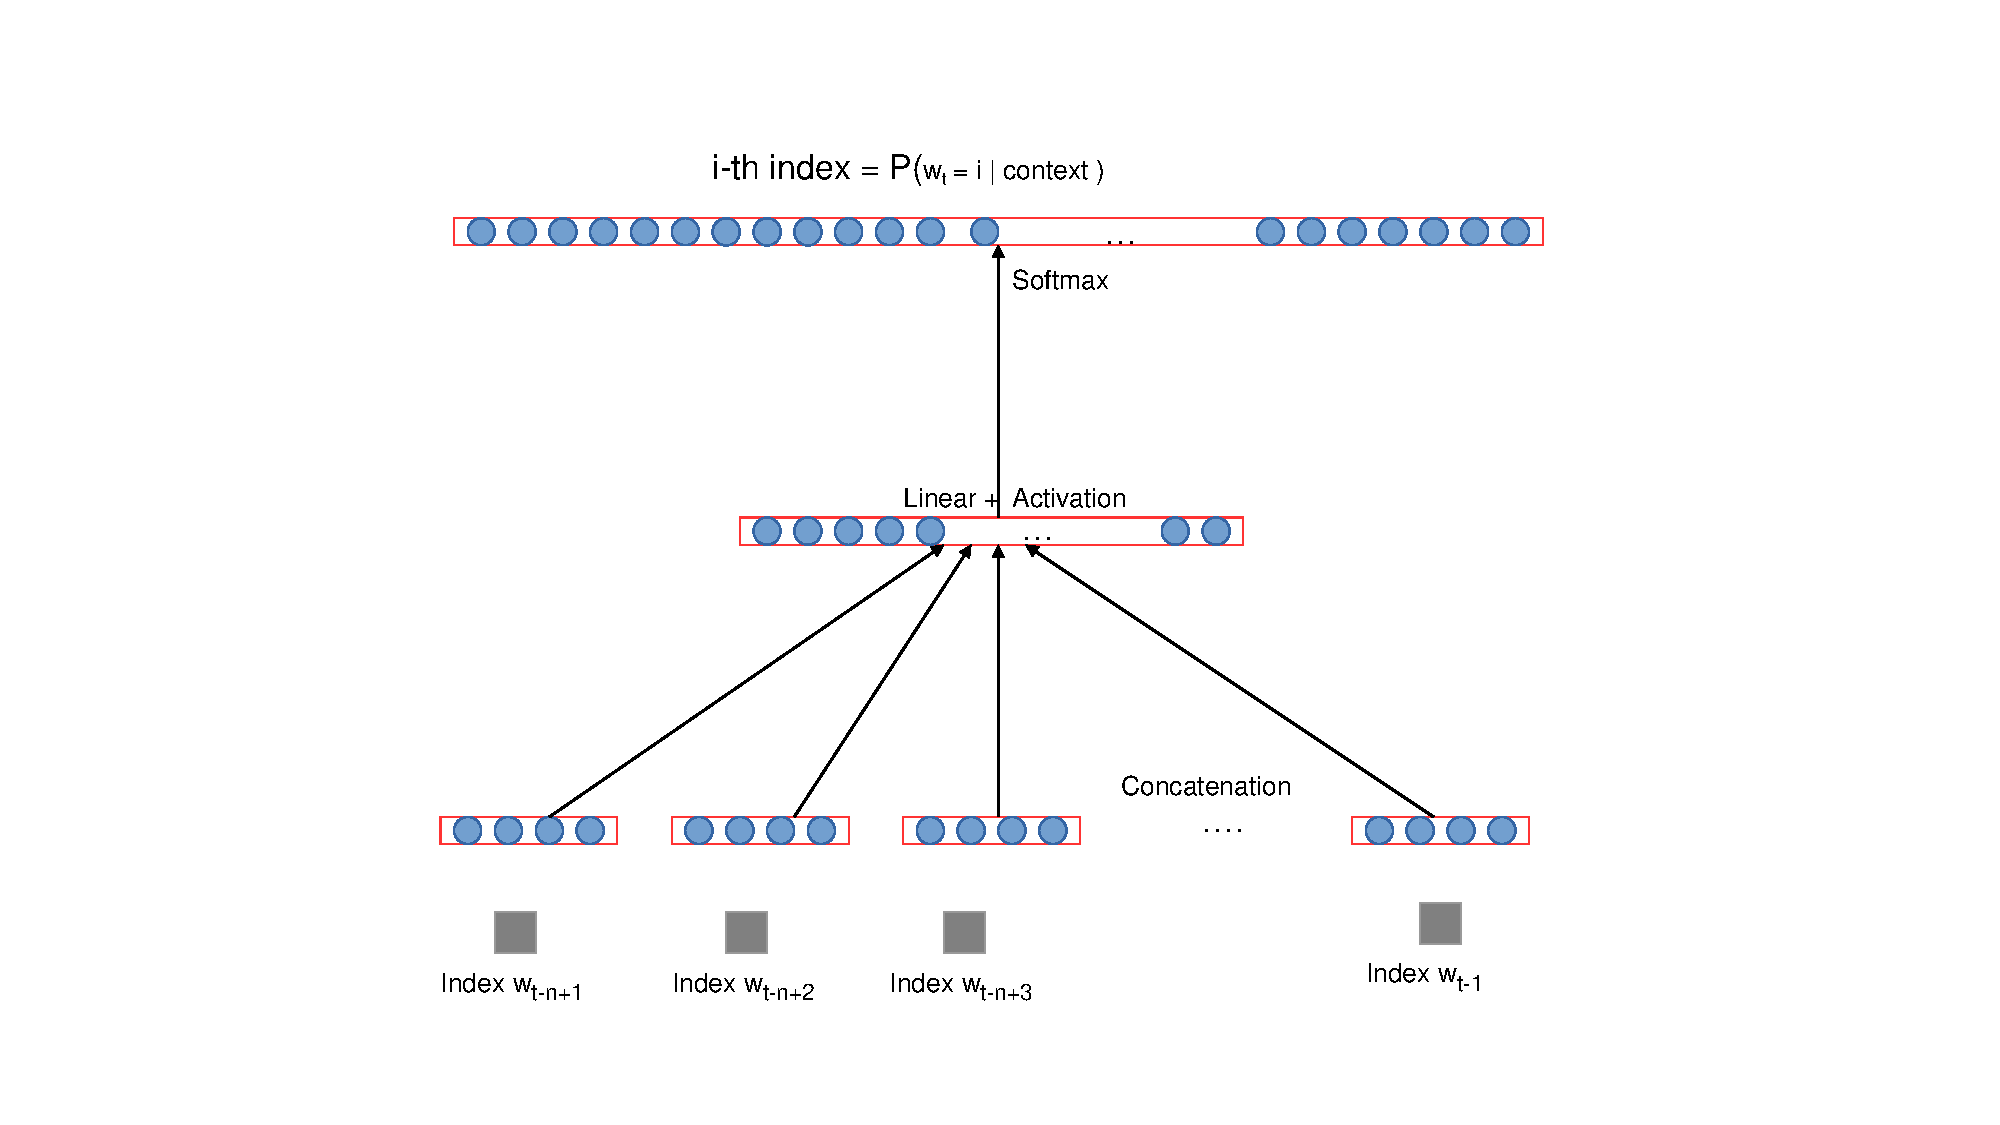
\includegraphics[width=\columnwidth]{figures/neuralLM.pdf}
~ \caption{Neural Language Model by Bengio et al~\cite{bengio2003neural}.}  
~ \label{fig:neuralBengio}
~ \end{figure}

\paragraph{Input layer}
The input layer constructs the embeddings of the words in the context, by using a shared word space and mapping each word in the context to a real-valued vector. Concretely, each word $w_i$ is represented as an 1-of-V coding, which is a long vector with the size of vocabulary V with all zeros except for the element corresponding to the word's index in the dictionary. Using this form of sparse coding, the word space (also called projection matrix $R$) is a matrix that contains V rows and each word embedding $v_i$ corresponds to one row of the matrix. The number of columns of the matrix is the size of the embedding, which is a tunable hyper-parameter. Notably, the values of the word vectors do not depend on the position of the word in the context. The context vector $i$ is the concatenation of the word vectors.

\begin{equation}
\begin{aligned}
i = \{R^T v_1; R^T v_2; .... ; R^T v_{n-1} \}
\end{aligned}  
\end{equation}


\paragraph{Hidden layer}
In the hidden layer, the input (context vector) is transformed nonlinearly, where each layer activation values are defined by

\begin{equation}
\begin{aligned}
h^j_{out} = f(W^j h_{in} + b^j) \\
h^1_{in} = i
\label{eq:hidden1}
\end{aligned}  
\end{equation}

In equation~\ref{eq:hidden1}, each hidden layer $h^j$ has the corresponding weights $W^j$ and $b^j$. The input of the first hidden layer is the context vector produced from the input (projection) layer. The size of the subsequent hidden layers are tunable hyper parameters. $f$ denotes a nonlinear activation function. Popular choices for the activation function are Tangent Hyperbolic, Sigmoid or ReLU, expressed in equation~\ref{eq:activation}. 


\begin{equation}
\begin{aligned}
 f(x) = 
	\begin{cases}
	\frac{\exp (x) - \exp (-x)}{\exp (x) + \exp (-x)}    \text{    if } f = \text{Tanh} \\
	\frac{1}{1 + \exp(-x)}                \text{     if } f = \text{Sigmoid} \\
	\max(0, x) \text{     if } f = \text{ReLU} \\
	\end{cases}
\label{eq:activation}
\end{aligned}
\end{equation}

\paragraph{Output layer}
The final layer of the network produces the probability distribution for all words in the vocabulary, thus having totally V nodes. Each neuron in the layer is associated to the probability of one word, as shown in Figure~\ref{fig:neuralBengio}. First, a linear transformation is used to obtain the unnormalised distribution:

\begin{equation}
\begin{aligned}
o = W^o h + b^o
\label{eq:linearoutput}
\end{aligned}  
\end{equation}

Notably, the values of $o$ is unnormalised because each element in o is associate to the score of each output word given the context vector. $W^o$ and $b^o$ are the corresponding weights and biases of the layer. Importantly, $W^o$ has the same form as the projection matrix at the input layer, since it also learns embedding for each word in the output vocabulary. Subsequently, the true probability distribution is estimated thanks to the~\textit{softmax} function:

\begin{equation}
p(w_i | h) = \frac{\exp(o_i)}{\sum_j \exp(o_j)}
\label{eq:softmax}
\end{equation}

In equation~\ref{eq:softmax}, the probability of each word $w_i$ given the encoded context $h$ is estimated by normalizing all values in $o$. Overall, the main tunable hyper-parameters of the network are the order of $n$-grams (the number of words in the context, which can range from 6 to 15), the sizes of hidden layers, and the word embedding size. The free parameters~$\Theta$ that are algorithmically learned from the data includes the projection matrix $R$, the weight matrices $W^h$ at the hidden layers, $W^o$ at the output layer and the biases $b^h$, $b^o$. 


\subsection{Training method}
From the machine learning perspective, the neural network language model has transformed the statistcal language modeling problem from a generative learning process to a discriminative classification problem. The free parameters of the network are trained by minimising the objective function, which is the log-likelihood~$\mathcal{L}$ of the  parameters~$\Theta$ given the training samples. The parameters are updated after each iteration based on some optimization techniques, among which Stochastic Gradient Descent (SGD) is most commonly used in neural language models \cite{zaremba2014recurrent,le2011structured,mikolov2010recurrent}. SGD and other variants such as Adadelta~\cite{zeiler2012adadelta} or RMSProp~\cite{tieleman2012lecture} require the computation of the first order derivatives of the loss function with respected to the parameters, which can be performed efficiently with the back-propagation algorithm~\cite{le1990handwritten}.

\subsection{Optimisation Process}
In this section, we describe the back-propagation flow in the standard feed forward neural language model - the core of the optimisation process. Back-propagation~\cite{rumelhart1985learning} involves using a dynamic programming strategy to compute the derivatives of the loss function with respect to the parameters layer by layer, based on the chain rules. In the standard network, the error derivatives are back-propagated from the output layer to the input (projection) layer.

\paragraph{Objective Function}

The smoothing function that we approximate with the neural network has parameters that can be iteratively tuned in order to~\textbf{maximise the log-likelihood of the training data}. 

The network aims at maximising the probability of the label word given the context, hence the objective function is typically chosen as the Negative Log-Likelihood function. Assuming we have N samples, each of which is an $n$-gram, we can compute the loss function over the training data as follows:

\begin{equation}
\mathcal{L} = - 	\sum_{i}^N \ln P( w_i | w_{i-n+1}^{i-1} ) \\
\label{eq:objective}
\end{equation}

The objective function is in line with the perplexity that we want to minimise (which is equivalent with maximising the log-likelihood of the training data). For ease of understanding, we denote the derivative of the loss function~$\mathcal{L}$ at~\textit{each} sample or batch of samples with respect to a variable $x \in \Theta$ by $dx$.  

For each sample, let's $w$ be the index of the predicted word $w_i$ in the vocabulary, we have:

\begin{equation}
\begin{aligned}
- \log P(w_i |  w_{i-n+1}^{i-1})  = - \log P(w | h) \\
= - log (\frac{\exp (o_w)}{\sum_i exp(o_i)}) \\
=  log(\sum_i \exp(o_i)) - o_w
\label{eq:objective2}
\end{aligned}
\end{equation}

Subsequently, we compute the error derivatives $dx$ given the parameters in each layer using back-propagation:

\paragraph{Output layer}

The derivatives at the output layer:

\begin{equation}
do_i = 
\begin{cases}
1 - p_i \text{ if } i == w \\
-p_i \text{     otherwise}
\end{cases}
\end{equation}

Notably, $o_i$ denotes the $i^{th}$ element of the vector $o$, which is the unnormalised distribution of the vocabulary given the encoded context $h$. 

\paragraph{Hidden layers}
As a result, we can compute the derivatives with respect to the parameters and the previous hidden layer $h$, based on the original inference from Equation~\ref{eq:linearoutput}. 

\begin{equation}
\begin{aligned}
dW^o = doh^T \\
db^o = do \\ 
dh = {W^o}^Tdo \\
\end{aligned}
\end{equation}


For the inner hidden layers, the  derivatives for the linear components are computed similarly, by replacing $do$ with $dh$ (the output of the previous hidden layer is the input of the next hidden layer). However, we have to take into account the non-linear activation functions, which are shown in the inference equation for the previous hidden layers:

\begin{equation}
h_{next} = f(W^h h_{prev} + b^h)
\end{equation}

With $W^h$ and $b^h$ are the corresponding weights connecting $h_prev$ to $h_next$. The derivatives are computed as follows:

\begin{equation}
\begin{aligned}
d[W^h h_{prev} + b^h] = f'(h_{next}) dh_{next} \\
db^h = d[W^h h_{prev} + b^h] \\
dW^h = d[W^h h_{prev} + b^h]h_{prev}^T \\
dh_{prev} = {W^h}^T d[W^h h_{prev} + b^h]
\label{eq:dhidden}
\end{aligned} 
\end{equation}

The derivative function of $f$, $f'$:

\begin{equation}
\begin{aligned}
f(x) = 
\begin{cases}
1 - \text{Tanh}(x)^2   \text{    if } f = \text{Tanh} \\
\text{Sigmoid}(x) - \text{Sigmoid}(x)^2                \text{     if } f = \text{Sigmoid} \\
1 \text{ when } x > 0 \text{ and 0 otherwise}  \text{     if } f = \text{ReLU} \\
\end{cases}
\label{eq:dactivation}
\end{aligned}
\end{equation}


\paragraph{Input Layer}

The derivative function of the input layer is identical to Equation~\ref{eq:dhidden} and Equation~\ref{eq:dactivation}, considering that the input layer is the layer before the first hidden layer. 

\paragraph{Parameter Update}

After obtaining the derivatives of the loss function with respect to all parameters in the network, we can update the parameters following Stochastic Gradient Descent. The method is based on the phenomenon that the gradient of a function always points towards the direction of maximal increase at any point. The update rule is as follows with the learning rate parameter $\alpha > 0$:

\begin{equation}
x = x - \alpha dx
\label{eq:sgd}
\end{equation}

The learning rate is also considered as a function of the number of samples trained in the data. Typically, the learning rate is updated after the model observes a number of training examples, with two most common ways. The first way is to exponentially decrease the learning rate after some training samples with a~\textit{learning rate decay}, normally an epoch (training all samples in the training data). The second way is to reduce the learning rate based on a validation data. After each epoch, if the perplexity on the validation data is decreased, the learning rate is kept the same, otherwise it is multiplied by the learning rate decay.


\subsection{Recurrent Neural Language Models}

Compared to the statistical $n$-gram models, the feed-forward neural language models had created a considerable leap in representation by combining distributed representation of words with a robust classifier to generalise from observed sequences. As can be seen from various works~\cite{schwenk2007continuous,le2011structured}, the feed-forward language model significantly outperformed the traditional Knesey-Ney back-off models. However, the feed-forward models require a fixed input size, thus still rely on the Markov Assumption which limits the context to a particular number of words, even when the context size can be huge up to $10$. In order to model long sentences, or even paragraphs with long-term dependencies, it is beneficial to investigate in models that can be flexible in terms of input size. For example, if the distance between the open bracket and the closed counterpart is further than the $n$-gram input size, the feed forward model may forget to close the brackets after seeing the initial one. Ideally, as the learning process of human is associated with a memory that keeps the current information (such as topics), similar structure should be simulated and integrated in the network.

\paragraph{Recurrent Neural Networks} RNN~\cite{elman1990finding} are a class of neural networks that can efficiently model sequences by using a dynamic memory structure. While the feed-forward network can only receive one input and compute the corresponding output without any relation with other inputs, the recurrent counterpart takes the input as a~\textit{series of time step}  $x_1, x_2, \dots, x_n$ and processes them one by one, taking into account the information stored in the previous steps. Concretely, for each input $x_i$, the network updates the hidden memory $h_i$ based on the previous one $h_{i-1}$. 

%The ''Vanilla`` model~\cite{elman1990finding} uses a simple combination of the input and the previous memory:

\begin{equation}
h_i = \mathcal{F}(x_i, h{i-1})
\end{equation}

 We will cover some popular RNN variations in the upcoming sections. In general, the strong point of these models lie in the ability to dynamically model sequences with arbitrary length, which the feed-forward neural networks cannot achieve. The advantage comes with the cost that the recurrent models are generally hard to train, due to the properties of back-propagation. A change in an arbitrary position of the sequence can lead to a change in the objective function, therefore training methods for RNNs typically have to trace back the previous time steps. In other words, the RNNs are equivalent to feed-forward neural networks with many hidden layers that share parameters across each other. Importantly, the model capacity of RNNs do not depend on the length of the sequences, but in the recurrence mechanism - the way the hidden layers are updated. 
 
\paragraph{Recurrent Language Models} Language Modeling can be viewed as a sequence modeling problem, in which each time step corresponds to one word. The first recurrent language model (RNNLM)~\cite{mikolov2010recurrent} employed the ``Vanilla'' model of Elman et al~\cite{elman1990finding} as can be seen in Figure~\ref{fig:SimpleRNN}, in which the hidden steps are updated as follows:

~ \begin{figure}[!t]
	~ \centering
	~ 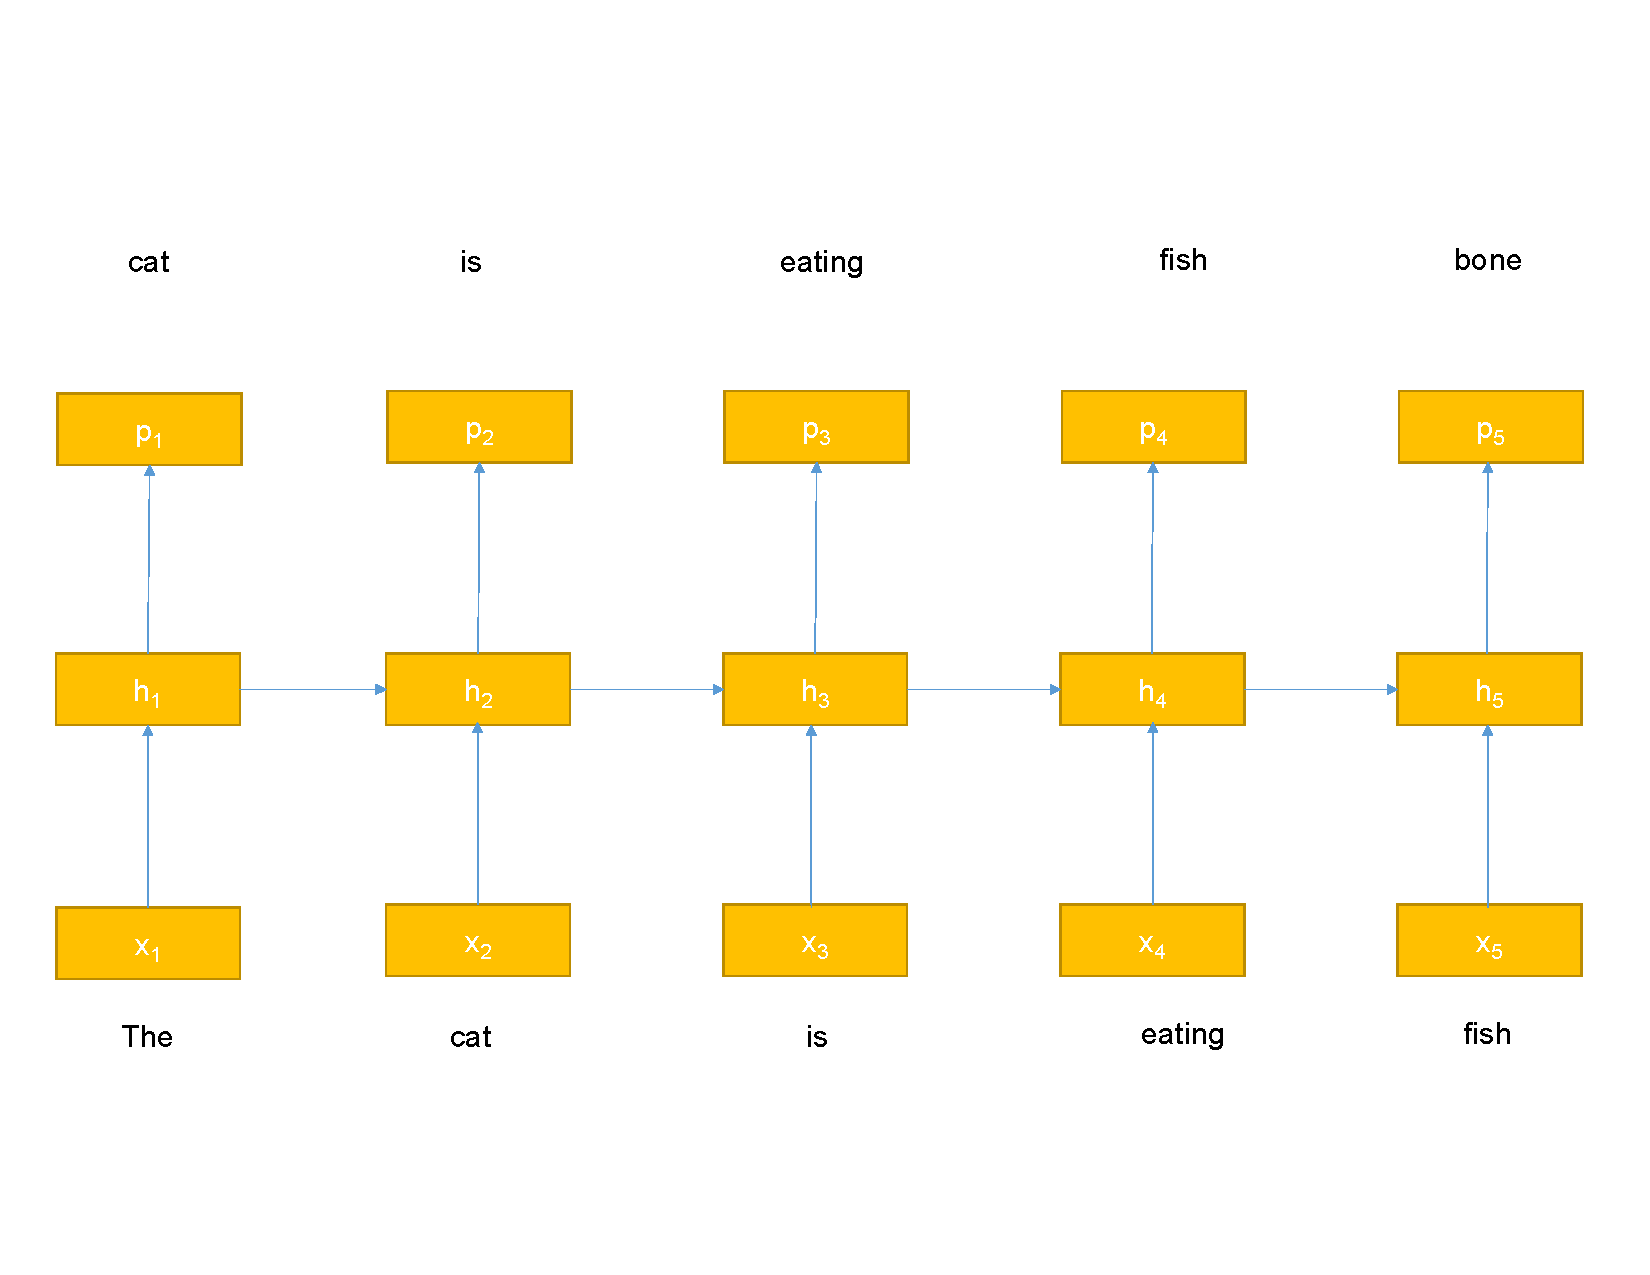
\includegraphics[width=\columnwidth]{figures/rnn.pdf}
	~ \caption{A simple RNNLM~\cite{mikolov2010recurrent} predicting the sequence ``The cat is eating fish bone''.}  
	~ \label{fig:SimpleRNN}
	~ \end{figure}


\begin{equation}
h_i = f(Wx_i +  Uh{i-1} + b)
\end{equation}

The activation function $f$ can be either Tangent Hyperbolic, Sigmoid or ReLU as mentioned before. The starting state $h_0$ is set to 0 to denote the initial state of the memory. In each time step, the RNNLM can optionally produces the probability distribution for a predicted word, given the sequence that network has scanned previously. The probability distribution over the vocabulary is derived similarly to the feed-forward networks:

\begin{equation}
\begin{aligned}
o_i = W^oh_i + b^o \\
p_i = \text{softmax}(o_i)
\end{aligned}
\end{equation}

with the Softmax function explained in Equation~\ref{eq:softmax}. To be clear, $o_i$ and $p_i$ denote the unnormalised and normalised distribution generated at time step $i$. For the language modeling scenario, the input and output samples of the network in each training iteration are two sequences $X \text{ and } Y$ in which the output sequence is the shift-by-1 version of the input sequence. The parameter set of the network including $W, b, U, W^o \text{ and } b^o$ are shared across time steps. 


\subsubsection{Training Recurrent Networks}

Similarly to the feed-forward models, The recurrent models can also be efficiently trained with stochastic gradient descent (SGD). However, since the networks contain shared parameters at arbitrary numbers of time steps, the gradients are computed differently using back-propagation through time (BPTT). The details of this algorithm are divided into two parts: the local gradients computed  at each time step, and the global gradients accumulated by un-folding the networks. 

\paragraph{At each time step}

% How to compute the gradients

\paragraph{For global derivatives}

Backpropagation through time algorithm 

\paragraph{Problems with BPTT}

Although truncated back-propagation through time provides a practical training method for RNNs, the nonlinear iterative nature of the simple RNN architecture still makes capturing long-term dependencies difficult. The two common problems encountered while training RNNs are the~\textit{exploding} and the~\textit{vanishing} gradients~\cite{bengio1994learning,pascanu2013difficulty}. On the one hand, the gradients can be exponentially large as in the back-propagation through time process which is detrimental for learning. One the other hand, we can also experience the phenomenon that gradients go quickly towards zero after being propagated through time steps. Consequently, the model is not able to track the signal and complete loses the memory trace in the past. For example, the original RNNLM normally has to truncate the BPTT at about $5-10$ steps, which has the same modeling capacity and performance with $10$-gram feed-forward models~\cite{mikolov2011extensions,hai2012measuring}. The gradient exploding problem can be tackled adequately using gradient clipping. Pascanu et al~\cite{pascanu2013difficulty} suggested to clip the norm of the gradients (for all parameters): given a gradient vector $dx$ that is computed with BPTT, if the norm $||dx||$ is greater than a threshold value $\delta$, then $dx$ would be softly scaled:

\begin{equation}
dx \leftarrow dx\frac{||dx||}{\delta}
\end{equation}

%Explain mathematically
\paragraph{Dealing with gradient vanishing}

A number of solutions were proposed to solve the gradient vanishing problem. We will make a brief review of the most prominent approaches. First, Mikolov et al~\cite{mikolov2014learning} proposed to integrate another memory layer which is formed by the bag-of-word addition of the input words over time, decays slower than the main hidden memory and is initialised as an identity matrix. The same initialisation trick is applied together with using Rectified Linear Units (ReLU) as the activation function in~\cite{le2015simple}. While both works mentioned are fairly simple, the RNNs can also be trained efficiently with second order derivatives using Hessian-Free optimization~\cite{martens2011learning}. Even though the method was prove to allow the network to acquire a reliable memory which can remain stable after hundreds of time steps, it is not easy to implement efficiently compared to traditional back-propagation. The most successful method that is applied to sequential modeling in general and language modeling in particular is the Long-Short Term Memory LSTM networks~\cite{hochreiter1997long} that use an explicit memory cell combined with a gating mechanism to intensively deal with the gradient vanishing problem.

\paragraph{LSTM Structure} The intuition of an LSTM starts from the integration of a linear memory unit, so that the gradient can flow smoothly during the back-propagation through time steps using a memory cell $c_t$. 

\begin{equation}
c_t = c_{t-1} + f(Wx_i +  Uh{i-1} + b)
h_t = c_t
\end{equation}

This approach is referred as ``Leaky integration units''~\cite{bengio2013advances}. In the BPTT process, the gradient can flow over exactly one path through the memory units $c_i$, and since $dc_i = dc_{i-1}$, the gradients are guaranteed to not vanish. The recurrent architecture should also be able to be adequately robust to train long sequences, where there are certain inputs which are irrelevant to the modeling task. Sometimes, the memory of the network should be refreshed, for example at the beginning of a new utterance in Speech Recognition~\cite{graves2005framewise} or a new sentence in Machine Translation~{sutskever2014sequence}. Hochreiter et al~\cite{hochreiter1997long} enhanced the architecture by adding flexible and trainable gates that allows the RNN to reset the memory, control the amount of input and output respectively. The adaptive gates are built from the current input $x_t$ and the previous hidden memory $h_t$. 

The gates of the network include: the forget gate $f_t$ is used to directly control the memory flow $c_t$ to cut the connection with the previous steps, the input gate $i_t$ decides the amount of input to be incorporated, the output gate $o_t$ controls the amount of memory flow to be produced for the task and finally the candidate memory unit $\tilde{C}$ that contributes to the current memory flow. All gates are defined similarly, with the first three gates use the Sigmoid activation to force the values to be in \{0, 1\}, while the candidate memory uses the Tanh activation function.

\begin{equation}
\begin{aligned}
f_t = \text{Sigmoid}(W_fx_t + U_fh_t + b_f) \\
i_t = \text{Sigmoid}(W_ix_t + U_ih_t + b_i) \\
o_t = \text{Sigmoid}(W_ox_t + U_oh_t + b_o) \\
\tilde{C}_t = \text{Sigmoid}(W_cx_t + U_ch_t + b_c) \\
\end{aligned}
\label{eq:lstm1}
\end{equation}

In the next step, we decide the new information to be stored in the new memory cell. The cell is updated by combine the input gate and the candidate memory unit. Also, the forget gate is employed to drop certain information from the previous memory cell. Consequently, we come up with a new memory cell as follows:

\begin{equation}
C_t = f_t * C{t-1} + i_t * \tilde{C}_t
\label{eq:lstm2}
\end{equation}

Finally, we update the hidden state with the new cell state and the output gate:

\begin{equation}
h_t = o_t * \text{Tanh}(C_t)
\label{eq:lstm3}
\end{equation}

In Equations~\ref{eq:lstm2} and~\ref{eq:lstm3}, the symbol $*$ denotes element wise matrix multiplication. The implementation of LSTM can be efficient by computing all gates in one single matrix multiplication, then applying the activation functions on different parts of the output. In practice, one can experience different implementation variations of LSTMs and RNNs in terms of initialisation, bias usage or different gate implementations such as the Gated Recurrent Unit~\cite{cho2014learning}. The empirical research of~\cite{zaremba2015empirical} shows that there is not any substantial difference in terms of performance between different LSTM variations. 

\paragraph{Training LSTM}

Rewrite the Backpropagation through time from RNN
%
%\section{Analysis}
%
%
%\subsection{Computational Complexity}
%
%\textbf{Bottleneck in the Softmax layer}
%
%\textbf{Approximating the Softmax}

%\section{Analysis}
%
%The most important achievement of neural network language models is the ability to model word representations with low dimension embeddings that can capture syntactic and semantic properties of words~\cite{mikolov2013distributed,mikolov2013efficient}. Such ability is trained simultaneously with the classifier in order to capture linguistic regularities, which helps the network to generalise over observed sequences. 
%
%Despite the fact that the state-of-the-art language models consist of a shared projection space between words, they still treat the context as a sequence of discrete symbols. The feed-forward network simply concatenate the word vectors and learn the non-linear mapping functions to get word combinations, while the recurrent models take one word as a time step, whose weakness is that a particular time step does not have any information about future steps. In fact, it is useful to take into account the collocations and multi-word expressions in the context. For example, the English word ``get'' can acquire different meanings when paired with different propositions, which the word embeddings hardly can represent. 
%
%Such word combinations are often identified by statistical methods~\cite{sag2002multiword}, which requires an intensive scanning through the data to find frequent combinations. In the context of the neural networks, it is intuitive to use a special neural network layer that has the~\textit{convolution} property, which goes through the input sequence by scanning with a small window to find pattern features. 





%~ \chapter{``Copy'' Mechanisms}
%~ \label{c:copy}

%~ \chapter{Attention Mechanisms}
%~ \label{c:attention}
%~ \input{4-attention.tex}

%~ \chapter{Hybrid Neural Machine Translation}
%~ \label{c:hybrid}
%~ \input{5-hybrid.tex}

%~ \chapter{Towards the Future of NMT}
%~ \label{c:future}
%~ \input{6-future.tex}

%~ \chapter{Conclusion}
%~ \label{c:conclude}
%~ \input{7-conclude.tex}


% -- Appendix --
\appendix


\bibliographystyle{plainnat}
\bibliography{thesis}
\end{document}
